\documentclass[a4paper]{article}
% Pacotes necessários
\usepackage[portuguese]{babel}
\usepackage[backend=biber, style=apa, citestyle=apa, language=portuguese]{biblatex}
\usepackage{csquotes}
\addbibresource{Recursos/referencias.bib}

\usepackage{amsmath}
\usepackage{graphicx}
\usepackage{subcaption}
\usepackage{setspace}
\usepackage{siunitx} % Required for alignment
\sisetup{
  round-mode          = places, % Rounds numbers
  round-precision     = 2, % to 2 places
}
\usepackage{enumerate}
\usepackage{enumitem}
\usepackage{amsmath}
\usepackage{karnaugh-map}
\usepackage[section]{placeins}
\usepackage{geometry}
\usepackage{amssymb}
\usepackage{titling}
\usepackage[T1]{fontenc}
\usepackage{float}
\usepackage[hidelinks]{hyperref}
\usepackage{xcolor}
\usepackage{indentfirst}
\usepackage{array}
\usepackage{soul}
\usepackage{afterpage}
\newcolumntype{P}[1]{>{\centering\arraybackslash}p{#1}}

% Comando para criar uma página vazia
\newcommand\myemptypage{
    \null
    \thispagestyle{empty}
    \addtocounter{page}{-1}
    \newpage
}

% Página de título principal
\newcommand{\firsttitlepage}{
    \begin{titlepage}
        \centering
        \vspace*{1cm}
        
        % Logos superior
        \begin{figure}[h!]
            \centering
            
\includegraphics[width=6cm]{Recursos/LOGO_IPB} % Substitua pelo caminho da imagem
            \vspace{0.5cm}
        \end{figure}

        % Informações da instituição
        \large\textbf{INSTITUTO POLITÉCNICO DE BEJA} \\
        \large\textbf{Escola Superior de Tecnologia e Gestão} \\
        \large\textbf{Licenciatura em Engenharia Informática} \\
        \large\textbf{Sistemas de Informação} \\
        
        \vspace{2cm}
        
        % Título do projeto
        {\Huge \textbf{Trabalho de Grupo 1}} \\
        
        \vspace{1.5cm}
        
        % Autores
        \large Martinho José Novo Caeiro \\
        \large Paulo António Tavares Abade \\
        
        \vfill
        
        % Logo inferior
        \begin{figure}[h!]
            \centering
            
\includegraphics[width=6cm]{Recursos/IPBejaESTIG.jpg} % Substitua pelo caminho da imagem
        \end{figure}
        
        \vspace{1cm}
        
        % Local e data
        {\large Beja, novembro de 2024}
    \end{titlepage}
}

\newcommand{\secondtitlepage}{
    \begin{titlepage}
        \centering
        \vspace*{1cm}
        
        % Informações da instituição
        \large\textbf{INSTITUTO POLITÉCNICO DE BEJA} \\
        \large\textbf{Escola Superior de Tecnologia e Gestão} \\
        \large\textbf{Licenciatura em Engenharia Informática} \\
        \large\textbf{Sistemas de Informação} \\
        
        \vspace{2cm}
        
        % Título do projeto
        {\Huge \textbf{Trabalho de Grupo 1}} \\
        
        \vspace{1.5cm}
        
        % Autores
        \large Martinho José Novo Caeiro \\
        \large Paulo António Tavares Abade \\
        
        \vfill
        
        % Local e data
        {\large Beja, novembro de 2024}
    \end{titlepage}
}

\begin{document}
\pagenumbering{gobble} % Oculta numeração da página

% Primeira página de título
\firsttitlepage

\secondtitlepage

% Início do conteúdo do relatório
\newpage
\doublespacing
\tableofcontents
\doublespacing

\newpage
\pagenumbering{arabic}

\section{Introdução}\label{intro}
Neste trabalho irá ser abordado com a Crise do Petróleo influenciou a produção e desenvolvimento
dos carros entre os anos 1970 e 1980, alterando o motor e por consequência a sua aceleração, eficiência e consumo.

Para analisar esta situação foi utilizada uma base de dados com 393 entradas, com 9 atributos iniciais, sendo estes:
 Milha por Galão, Cilindros, Cilindrada, Cavalagem, Peso, Aceleração, Ano de Fabrico, País de Origem e o Nome Completo do Carro.

Ainda foi utilizada outra base de dados que indica o preço médio de combustível por ano, entre 1970 e 1982, 
nos Estados Unidos da América.

Por fim, a nossa teoria é que a Crise do Petróleo influenciou a produção e 
desenvolvimento dos carros entre os anos 1970 e 1980, alterando o motor e por consequência a sua aceleração, eficiência e consumo.

\section{Metodologia de Trabalho}\label{met}
Para o desenvolvimento deste trabalho foi utilizado o \textit{Github} para a partilha de código e documentação,
o \textit{Visual Studio Code} como IDE de desenvolvimento, o \textit{Excel - PowerQuery} ferramenta principal de tratamento
e análise de dados e por fim, o \textit{SQL Server Managment} para a criação da Dataware House. 

\section{ETL}\label{etl}
O trabalho de ETL foi realizado em 3 fases, a primeira foi a extração dos dados, 
a segunda a transformação e por fim a inserção dos dados em tabelas dinâmicas.

\subsection{Extração de Dados}
Os dados foram extraídos de um ficheiro \textit{.csv} que foi encontrado no Kaggle (\cite{kaggle}) e 
importados para o \textit{Excel} utilizando o PowerQuery.

\subsection{Transformação de Dados}
Com o auxílio do PowerQuery foi possível transformar os dados, e foram encontrados diversos problemas,
como por exemplo, a presença de valores nulos, duplicados e a necessidade de alterar o tipo de dados de algumas colunas.
Ainda foram encontrados problemas com a formatação dos dados, como por exemplo, a presenção de vírgulas em vez de pontos.
O nome das colunas também foi alterado para facilitar a sua identificação e foram adicionadas novas colunas para facilitar a análise
e permitir a criação de tabelas dinâmicas, sendo que as novas colunas são: Marca e Modelo.

\subsection{Inserção de Dados}
Utilizando as tabelas dinâmicas do Excel, foi possível visualizar os dados de forma mais clara e objetiva, e foram separados da seguinte
forma: Geral e Especifíca.

\begin{figure}[h!]
    \centering
    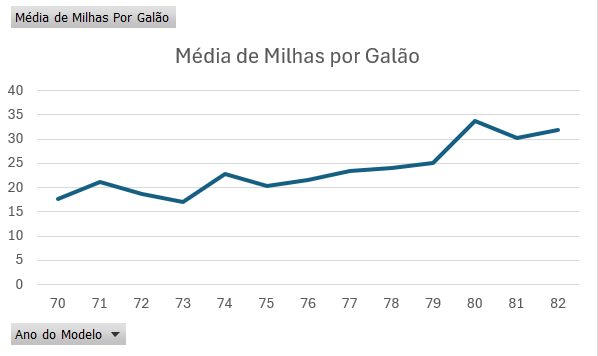
\includegraphics[width=6cm]{Recursos/MPG_Geral} % Substitua pelo caminho da imagem
    \vspace{0.5cm}
\end{figure}

\begin{figure}[h!]
    \centering
    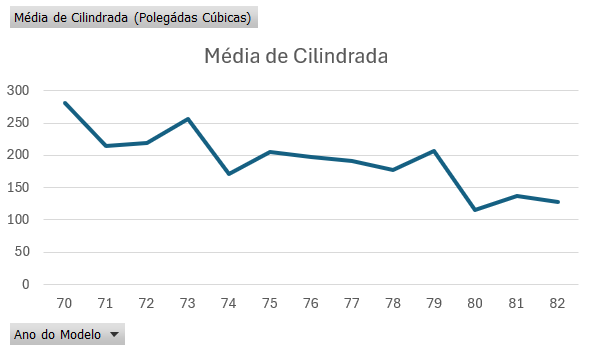
\includegraphics[width=6cm]{Recursos/MC_Geral} % Substitua pelo caminho da imagem
    \vspace{0.5cm}
\end{figure}

\begin{figure}[h!]
    \centering
    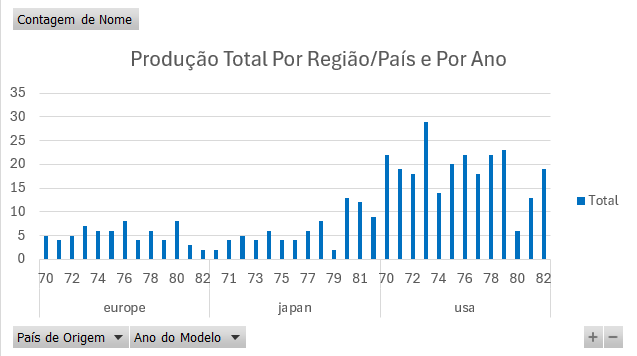
\includegraphics[width=6cm]{Recursos/Total_Geral} % Substitua pelo caminho da imagem
    \vspace{0.5cm}
\end{figure}

\subsubsection{Geral}

\subsubsection{Especifíca}


\section{Criação da Dataware House}\label{dwh}



\section{Contexto Global}\label{cg}
Texto sobre supercondutores.


\section{Conclusões e Perspectivas de Trabalho Futuro}\label{con}
Texto das conclusões.

\newpage
\renewcommand{\refname}{Bibliografia} % Para artigos
\renewcommand{\bibname}{Bibliografia} % Para livros e relatórios
\addcontentsline{toc}{section}{Bibliografia} % Adiciona a Bibliografia ao índice
\printbibliography

\end{document}
